\chapter{Analyse des données}


\section{Data Mining - Analyse exploratoire}

\subsection{Pre-processing}
%Description du dataset (rapidement, le reste dans un codebook)\\

%Mise en forme du dataset, une sortie à la fois vs plusieurs sorties etc \\
%On considère les données gustatives et les défauts physiques comme des sorties -> les prendre un par un ou tous ensemble\\

%Description du set, différentes parties des données, éventuelles données manquantes\\

Une grande partie de l'étape de préprocessing a été réalisée durant l'extraction des données. Il a en effet fallu extraire les données d'une manière uniforme et cohérente dès le départ afin de ne pas se retrouver avec des variables présentes uniquement dans certaines parties du set de données ou avec des variables incohérentes comme cela a été le cas de certains cafés qui avaient comme note de dégustation plus de cent points sur cent par exemple. Des éliminations ou des corrections ont été réalisées de manière automatisées ou manuelles afin de supprimer les erreurs. On notera parmi les corrections importantes le remplacement de virgules par des points, quelques erreurs de frappes (68.5 points sur 10 au lieu de 6.85 par exemple) ou encore des utilisations d'unités différentes. Le dataset résultant est décrit dans l'Annexe A de ce projet. Une fois cette étape de nettoyage réalisée, les premières informations ont pu être extraites des données.\\

%TODO Annexe A

\noindent Le schéma \ref{DatasetMaking} résume rapidement les différentes élimination d'observations au cours des étapes de construction du set de données. 

\begin{figure}[H]
	\includegraphics[scale=0.5]{Dataset_1}
	\caption{\label{DatasetMaking} Étape de construction du set de données et pertes d'observations.}
\end{figure}

%TODO Vérifier






\paragraph{Variables dépendantes\label{VarDep}} Les variables de sorties, ou dépendantes, sont composées des dix analyses de dégustation et éventuellement de la totalité des défauts physiques des grains. Sauf pour les défauts physiques des grains, qui sont éliminés avant la dégustation, les variables de sorties sont très corrélées entre elles et il a été discuté avec le responsable du comité  de sélectionner les variables les plus importantes. Ces variables sont \textit{Acidez}, \textit{Dulzor} et \textit{Puntaje Total} ainsi que la catégorie décrite dans le paragraphe suivant qui a été ajouté au set de données.  

\paragraph{Catégories}
Les cafés colombiens sont réputés excellents mais sur les 100 points attribuable lors des dégustations qu'est-ce que cela représente ? Le tableau \ref{categoriesCafe} nous donne une bonne idée de l'échelle représentée. Ces catégories seront utilisées dans le set de données pour tenter de réaliser une classification. 
\begin{table}[H]
	\centering
	\caption{Catégories de cafés d'après le nombre de points \newline Source: http://www.scaa.org/?page=resources\&d=cupping-protocols \label{categoriesCafe}}
	\begin{tabular}{llllcl}
		\textbf{Total Score}   &  & \textbf{Quality Classification}   & \textbf{Specialty or not}  & \textbf{Category} \\
		
		90-100        &  & Outstanding              & Specialty         &  1                    \\
		85-89.99      &  & Excellent                & Specialty         &  2                    \\
		80-84.99      &  & Very Good                & Specialty         &  3                    \\
		\textless80.0 &  & Below Specialty Quality & Not Specialty     &  4                   
	\end{tabular}
\end{table}



\paragraph{Élimination des résultats avec zéro points} Certain cafés du dataset ont zéro points en sortie pour chacune des 10 catégories notées. Il a été décidé de ne pas prendre en compte ces cafés lors des calculs de prédiction ou de clustering car la qualité du sol ou du climat ne peut justifier une telle baisse de qualité à elle seule dans une région réputée propice et qu'un défaut de traitement du grain, un mauvais tri avant la dégustation ou autre facteur externe doit en être la cause. Cependant, afin de se faire une idée d'éventuelles causes de cette qualité médiocre, les cafés sus-mentionnés ont été gardés pour la réalisation des cartes SOM au chapitre \ref{SOM}. 





\subsection{Analyse exploratoire}


\subsubsection{Emplacement des fermes}\label{EmpFermes} L'emplacement des différents cafés par rapport aux nombre de points est présenté sur la figure \ref{FincaVSPoints}. La catégorie 1 (non représentée) correspond aux cafés avec plus de 90 points, la 2 aux cafés avec plus de 85, la 3 aux cafés avec plus de 80 et la 4 aux cafés en dessous de 80, ne correspondant donc pas à la qualité "Specialty". On peut y voir que l'emplacement dans le département n'as pas d'incidence sur les résultats, la répartition des différentes classes étant très uniforme. 


\begin{figure}[H]
	\includegraphics[scale=0.59]{Map_North}
	\newline
	\newline
	\newline
	\includegraphics[scale=0.5]{Map_South}
	
	\begin{figure}[H]
		\includegraphics[scale=1]{Legend_Map2}
	\end{figure}
	\caption{\label{FincaVSPoints} Emplacement des fermes avec coloration selon le nombre de points attribués au café.}
\end{figure}


\subsubsection{Corrélations entre variables}

Afin d'avoir une bonne vue d'ensemble sur les variables et leurs liens, les matrices de corrélation ont été calculées pour toutes les variables. Premièrement la corrélation entre les différentes sorties. Sur la figure \ref{correlation_sorties1} on peut observer que les défauts physiques des grains ne sont que très peu liés entre eux ou avec les résultats de dégustation. On remarque cependant que les données gustatives du café sont fortement liées entre elles. 

\begin{figure}[H]
	\includegraphics[scale=0.35]{correlation_sorties1}
	\caption{\label{correlation_sorties1} Matrice de corrélation entre les différentes sorties.}
\end{figure}


\noindent Sur la figure \ref{correlation_all1} on peut observer les corrélations entre toutes les variables. 


\begin{figure}[H]
	\includegraphics[scale=0.35]{correlation_all1}
	\caption{\label{correlation_all1} Matrice de corrélation entre toutes les variables.}
\end{figure}


\noindent On observe que les données de sol sont parfois corrélées entre-elles mais presque pas du tout avec les données climatiques. On peut donc déjà soulever que le climat n'a pas ou peu d'influence sur la texture, le pH ou le taux de matière organique du sol des zones étudiées. Les précipitations ont une influence importante sur les défauts physiques des grains, en revanche nous n'avons aucune variable qui a une corrélation marquée avec les points totaux et donc la qualité du café.   



%TODO Parler des variétés de cafés et de quelques données les concernants (Moyennes de points, rendement par variété, altitude etc) 









%TODO vérifier la version -> ne pas inclure les données de sorties !
\newpage
\subsubsection{Principal Component Analysis (PCA) et Clustering}\label{PCAss}
La PCA, pour Analyse en Composantes Principales en français, est une méthode qui consiste à transformer un jeu de variables corrélées en nouvelles variables dé-corrélées les unes des autres. Ces nouvelles variables sont appelées composantes principales et permettent de rendre l'information moins redondante. Pour faire plus simple, l'utilité de la Composante Principale est de réduire le nombre de variables tout en gardant un maximum d'information. La figure \ref{PCAdefinition} montre une représentation graphique de la composante principale. 


\begin{figure}[H]
	\includegraphics[scale=0.5]{PCA_1}
	\caption{\label{PCAdefinition} Description de l'Analyse en Composante Principale. (A) Description d'un objet simple de manière compliquée ( trois dimensions pour par exemple une ellipse en papier) (B) Trouver des nouvelles variables (axes de coordonnées) orthogonaux l'un à l'autre qui pointent dans les directions de la plus grande variance (C) Utiliser les nouvelles variables (axes) pour décrire l'objet d'une manière plus simple. }
\end{figure}

\paragraph{Résultats de la PCA}

L'analyse sur une version compacte des variables a donné les résultats présentés dans le tableau \ref{TablePCAResult1} et sur la figure \ref{FigurePCAResult1}. Une première analyse avait été effectuée sur le set de données complet, c'est-à-dire avec la totalité des données climatiques et non les moyennes, et les résultats se sont avérés similaires mais plus difficilement lisibles. Il a donc été choisi de résumer les variables pour réaliser la PCA et le clustering. La PCA du tableau \ref{TablePCAResult} ne comprend pas les cafés avec zéro points.
\begin{table}[]
	\centering
	\begin{tabular}{lllllll}
		& PC1     & PC2     & PC3     & PC4     & PC5     & PC6     \\
		ASNM           & \textbf{0.4125}  & 0.0766  & -0.0360 & 0.1766  & -0.1337 & 0.0397  \\
		Luminosidad    & -0.0169 & 0.2320  & 0.1532  & -0.3178 & -0.2836 & 0.0157  \\
		PrecTotalAvg   & -0.1714 & 0.1424  & 0.0222  & \textbf{-0.6767} & -0.0667 & 0.0926  \\
		TminTotalAvg   & \textbf{-0.4589} & -0.0115 & 0.1086  & -0.1232 & 0.0013  & 0.0809  \\
		TmaxTotalAvg   & \textbf{-0.4745} & -0.0334 & 0.0296  & 0.1501  & -0.0253 & -0.0329 \\
		TmeanTotalAvg  & \textbf{-0.4803} & -0.0252 & 0.0631  & 0.0409  & -0.0149 & 0.0133  \\
		DtrTotalAvg    & -0.3323 & -0.0517 & -0.0884 & \textbf{0.4712}  & -0.0529 & -0.1769 \\
		OrientationNum & 0.0623  & 0.0592  & -0.0886 & -0.1839 & \textbf{0.3797}  & \textbf{-0.5662} \\
		Slope          & 0.0657  & -0.1842 & 0.1179  & 0.1047  & 0.0434  & \textbf{0.6905}  \\
		pH\_avg        & 0.0135  & 0.3892  & 0.3844  & -0.0168 & 0.1244  & 0.0679  \\
		org\_avg       & 0.0493  & 0.1781  & \textbf{0.5036}  & 0.2176  & -0.1639 & -0.1841 \\
		Franco         & -0.0157 & \textbf{0.5453}  & 0.1441  & 0.1921  & 0.1676  & 0.1108  \\
		Arcilloso      & -0.0180 & -0.3026 & 0.2993  & -0.0844 & \textbf{0.4532}  & 0.1751  \\
		Limoso         & -0.0754 & \textbf{0.5018}  & \textbf{-0.2016} & 0.1095  & 0.2726  & 0.1712  \\
		Arenoso        & -0.0210 & 0.0645  & 0.0180  & 0.0048  & \textbf{-0.6303} & -0.0156 \\
		Cascajoso      & 0.0760  & -0.2236 & \textbf{0.6130}  & 0.0095  & 0.0109  & \textbf{-0.2053}
	\end{tabular}
	\caption{\label{TablePCAResult1}Tableau des rotations des six premiers composants de la PCA avec mise en évidence des variables les plus importantes par composante.}
\end{table}


\begin{figure}[H]
	\includegraphics[scale=1]{pca_complete.pdf}
	\caption{\label{FigurePCAResult1} Résultats de la PCA sous forme graphique. Réalisé avec la totalité des variables }
\end{figure}


\paragraph{Analyse des composantes} Le tableaux \ref{TablePCAResult1} montre l'importance des variables dans les différentes composantes de la PCA réalisée avec un  jeu de variables simplifié pour plus de lisibilité, après vérification que l'importance des types de variables des deux tableaux était similaire. \\

\noindent La première composante met en évidence les températures par rapport à l'altitude alors que la deuxième et la troisième mettent en évidence principalement les caractéristiques du sol. La quatrième montre une dé-corrélation entre les précipitations moyennes et les DTR et la cinquième composante montre une corrélation entre la texture argileuse du sol et son orientation à l'opposé à d'un sol sablonneux. La sixième composante met en évidence une relation entre l'orientation et et les sols rocailleux à l'opposé des sols pentus. 


% https://georgemdallas.wordpress.com/2013/10/30/principal-component-analysis-4-dummies-eigenvectors-eigenvalues-and-dimension-reduction/

%https://onlinecourses.science.psu.edu/stat505/node/54
\paragraph{Clustering} Afin de vérifier la présence éventuelle de groupes d'individus parmi la population de café, nous réalisons un HCPC, pour \textit{Hierarchical Clustering on Principal Components}, à l'aide de la PCA. La figure \ref{HCT_Suggest} nous montre l'arbre hiérarchique créé ainsi que le nombre de cluster proposé. \\

\begin{figure}[H]
	\includegraphics[scale=0.45]{HierarchicalClustering_TreeAndSuggestedNbCluster.pdf}
	\caption{\label{HCT_Suggest} HCPC et proposition de nombre de cluster }
\end{figure}



\begin{figure}[H]
	\includegraphics[scale=0.7]{HierarchicalClustering3D.pdf}
	\caption{\label{HCT_3d} HCPC arbre 3D}
\end{figure}


\noindent La figure \ref{HCT_Inert} nous montre les sauts d'inertie du dendogramme. On peut y voir qu'entre 2 et 3 clusters nous avons un saut assez grand puis à nouveau entre 4 et 5 avant une stabilisation. 


%http://www.sthda.com/english/wiki/hcpc-hierarchical-clustering-on-principal-components-hybrid-approach-2-2-unsupervised-machine-learning

\begin{figure}[H]
	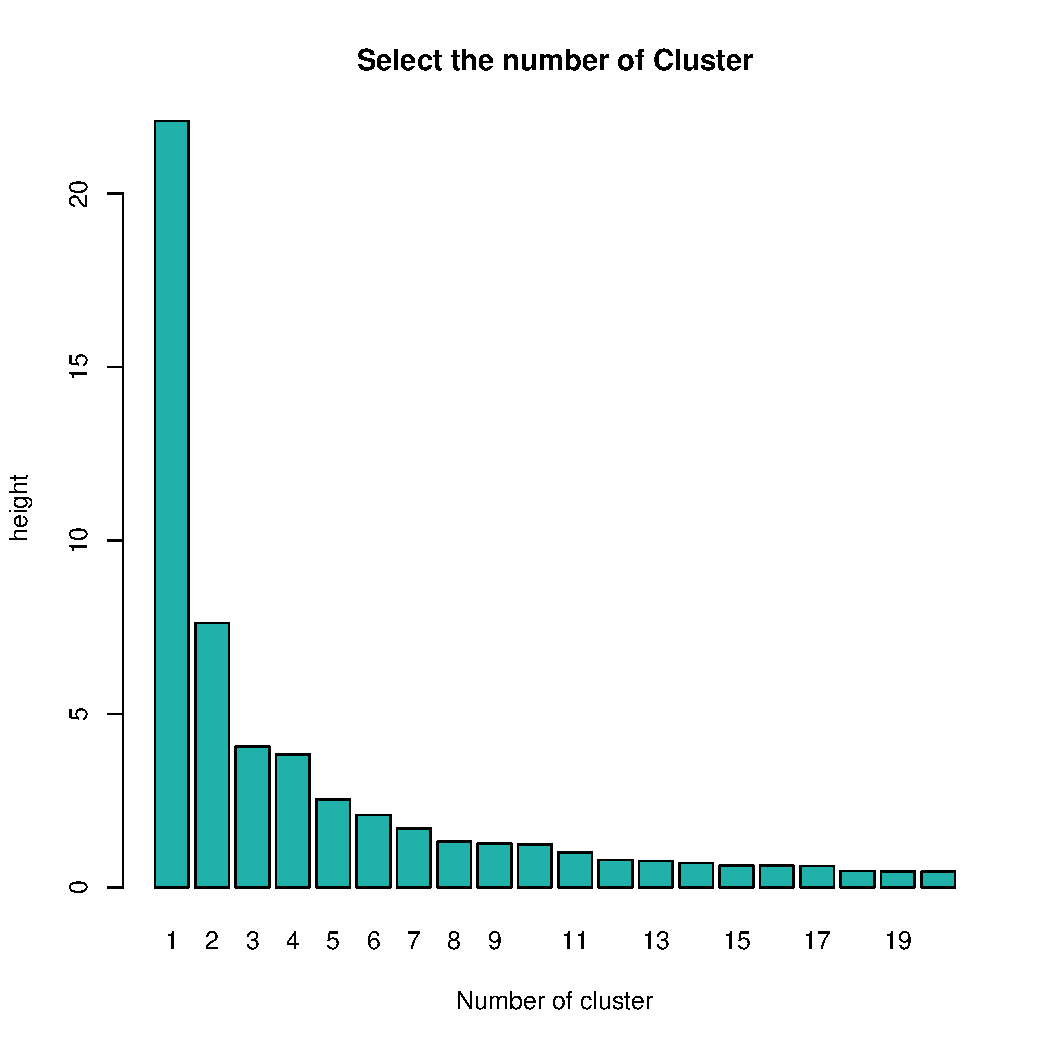
\includegraphics[scale=0.65]{NbClusterSelectInertiaGain.pdf}
	\caption{\label{HCT_Inert} Saut d'inertie du dendogramme  }
\end{figure}

%\noindent L'outil de HCPC nous fournit en sortie un objet de description des classes par les variables





\noindent L'ajout de clusters au set de données serait utile du moment que les clusters permettent significativement de séparer les types de cafés, au sens variables dépendantes du terme. Visuellement on devrait pouvoir observer une différence entre le nombre de café dans chaque cluster et les variables de sorties. Cependant ce n'est pas le cas comme on peut le voir ci-dessous: 


\begin{table}[H]
	\centering
	\label{cluster3category}
	\begin{tabular}{llll}
		 & 1  & 2  & 3   \\
		 \hline
		cat 2            & 0  & 28 & 21  \\
		cat 3            & 72 & 98 & 146 \\
		cat 4            & 44 & 70 & 157 
	\end{tabular}
	\caption{HCPC avec trois clusters comparés à la sortie catégories}
\end{table}



\begin{table}[H]
	\centering
	\label{cluster3acidez}
	\begin{tabular}{llll}
		& 1  & 2  & 3   \\
		\hline
		5    & 0  & 3  & 0   \\
		5.5  & 0  & 1  & 0   \\
		6    & 3  & 6  & 18  \\
		6.25 & 1  & 1  & 3   \\
		6.5  & 5  & 8  & 35  \\
		6.75 & 1  & 0  & 7   \\
		7    & 39 & 50 & 102 \\
		7.25 & 13 & 13 & 24  \\
		7.5  & 53 & 40 & 76  \\
		7.75 & 1  & 6  & 8   \\
		8    & 0  & 59 & 47  \\
		8.25 & 0  & 8  & 4   \\
		8.5  & 0  & 1  & 0  
	\end{tabular}
	\caption{HCPC avec trois clusters comparés à la sortie Acidez}
\end{table}


\begin{table}[]
	\centering
	\label{my-label}
	\begin{tabular}{llll}
		& 1  & 2  & 3  \\
		\hline
		42     & 0  & 0  & 1  \\
		49     & 0  & 1  & 2  \\
		50     & 0  & 3  & 0  \\
		52.5   & 0  & 0  & 1  \\
		58     & 0  & 0  & 1  \\
		58.5   & 0  & 1  & 0  \\
		59     & 0  & 2  & 0  \\
		59.5   & 0  & 1  & 0  \\
		60     & 0  & 3  & 2  \\
		60.5   & 0  & 2  & 0  \\
		61     & 1  & 0  & 1  \\
		61.75  & 0  & 1  & 0  \\
		62.5   & 0  & 0  & 1  \\
		63     & 0  & 1  & 0  \\
		64     & 0  & 0  & 1  \\
		65.5   & 0  & 0  & 1  \\
		66     & 0  & 1  & 1  \\
		67     & 0  & 1  & 4  \\
		68     & 1  & 0  & 2  \\
		68.75  & 0  & 1  & 0  \\
		69     & 0  & 1  & 1  \\
		69.5   & 0  & 0  & 1  \\
		69.75  & 0  & 0  & 1  \\
		70     & 0  & 0  & 1  \\
		70.75  & 1  & 0  & 0  \\
		71     & 1  & 2  & 3  \\
		71.375 & 0  & 0  & 1  \\
		71.75  & 0  & 1  & 0  \\
		72     & 0  & 1  & 2  \\
		72.5   & 0  & 1  & 0  \\
		72.75  & 0  & 0  & 1  \\
		73     & 0  & 5  & 3  \\
		73.25  & 0  & 1  & 0  \\
		73.5   & 0  & 0  & 2  \\
		74     & 0  & 0  & 2  \\
		74.75  & 0  & 1  & 1  \\
	\end{tabular}
	\begin{tabular}{llll}
		& 1  & 2  & 3  \\
		\hline
		74.875 & 0  & 0  & 1  \\
		75     & 1  & 2  & 2  \\
		75.25  & 1  & 0  & 4  \\
		75.375 & 0  & 0  & 1  \\
		75.5   & 1  & 3  & 2  \\
		75.75  & 0  & 1  & 2  \\
		76     & 2  & 2  & 8  \\
		76.125 & 0  & 0  & 2  \\
		76.25  & 0  & 0  & 2  \\
		76.375 & 1  & 0  & 0  \\
		76.5   & 4  & 3  & 6  \\
		76.75  & 1  & 0  & 4  \\
		77     & 4  & 3  & 8  \\
		77.25  & 0  & 1  & 2  \\
		77.5   & 1  & 0  & 3  \\
		77.75  & 1  & 2  & 5  \\
		77.875 & 1  & 0  & 0  \\
		78     & 7  & 4  & 3  \\
		78.25  & 0  & 1  & 1  \\
		78.5   & 1  & 1  & 7  \\
		78.75  & 0  & 0  & 2  \\
		79     & 13 & 10 & 41 \\
		79.25  & 1  & 3  & 5  \\
		79.45  & 0  & 0  & 1  \\
		79.5   & 0  & 2  & 4  \\
		79.52  & 0  & 0  & 1  \\
		79.625 & 0  & 0  & 2  \\
		79.75  & 0  & 1  & 1  \\
		80     & 6  & 7  & 8  \\
		80.25  & 0  & 1  & 4  \\
		80.375 & 0  & 0  & 1  \\
		80.5   & 2  & 1  & 8  \\
		80.625 & 1  & 0  & 0  \\
		80.75  & 1  & 2  & 8  \\
		81     & 4  & 0  & 6  \\
		81.25  & 1  & 3  & 6  \\
	\end{tabular}
	\begin{tabular}{llll}
		& 1  & 2  & 3  \\
		\hline
		81.375 & 1  & 0  & 1  \\
		81.5   & 3  & 3  & 8  \\
		81.625 & 1  & 0  & 1  \\
		81.75  & 1  & 1  & 9  \\
		82     & 7  & 4  & 13 \\
		82.25  & 7  & 2  & 4  \\
		82.375 & 2  & 0  & 2  \\
		82.5   & 29 & 24 & 19 \\
		82.75  & 5  & 3  & 4  \\
		83     & 0  & 10 & 14 \\
		83.25  & 0  & 3  & 5  \\
		83.5   & 1  & 7  & 6  \\
		83.75  & 0  & 3  & 3  \\
		84     & 0  & 5  & 8  \\
		84.25  & 0  & 5  & 2  \\
		84.5   & 0  & 8  & 5  \\
		84.75  & 0  & 6  & 1  \\
		85     & 0  & 7  & 6  \\
		85.25  & 0  & 4  & 0  \\
		85.5   & 0  & 1  & 2  \\
		85.75  & 0  & 3  & 4  \\
		86     & 0  & 4  & 1  \\
		86.25  & 0  & 0  & 1  \\
		86.5   & 0  & 3  & 2  \\
		86.75  & 0  & 1  & 3  \\
		87     & 0  & 1  & 2  \\
		87.25  & 0  & 2  & 0  \\
		87.5   & 0  & 1  & 0  \\
		87.75  & 0  & 1  & 0 \\
		&&&  \\
		&&&  \\
		&&&  \\
		&&&  \\
		&&&  \\
		&&&  \\
		&&&  
	\end{tabular}
\caption{Tableau des clusters pour la sortie Puntaje Total}

\end{table}

\begin{table}[H]
	\centering
	\label{ClusterVarImp}
	\begin{tabular}{lll}
		& Eta2       & P-value       \\
		\hline
		TmaxTotalAvg   & 0.79323282 & 8.808042e-216 \\
		TmaxTotal      & 0.79323282 & 8.808042e-216 \\
		tmean6         & 0.79308656 & 1.101237e-215 \\
		tmax6          & 0.77941800 & 6.561977e-207 \\
		TmeanTotalAvg  & 0.77802701 & 4.779121e-206 \\
		TmeanTotal     & 0.77802701 & 4.779121e-206 \\
		tmax7          & 0.77433881 & 8.706622e-204 \\
		tmean10        & 0.77341542 & 3.162373e-203 \\
		tmean5         & 0.77255468 & 1.047399e-202 \\
		tmean7         & 0.77146031 & 4.770308e-202 \\
		tmean9         & 0.76659843 & 3.682110e-199 \\
		tmax5          & 0.75947622 & 4.888995e-195 \\
		tmean8         & 0.75943990 & 5.127819e-195 \\
		tmax8          & 0.75506157 & 1.527633e-192 \\
		tmax9          & 0.73797359 & 2.717166e-183 \\
		tmin10         & 0.73685898 & 1.038321e-182 \\
		tmean4         & 0.72591249 & 4.041247e-177 \\
		tmax1          & 0.72445394 & 2.159972e-176 \\
		tmax4          & 0.72115391 & 9.274507e-175 \\
		tmax10         & 0.71764667 & 4.803959e-173 \\
		tmean1         & 0.71497543 & 9.398029e-172 \\
		tmin6          & 0.70461972 & 7.372790e-167 \\
		TminTotalAvg   & 0.68401310 & 1.306441e-157 \\
		TminTotal      & 0.68401310 & 1.306441e-157 \\
		tmean2         & 0.67984980 & 8.149567e-156 \\
		tmin8          & 0.67467087 & 1.293430e-153 \\
		tmax2          & 0.66718704 & 1.700396e-150 \\
		tmin9          & 0.66714064 & 1.776914e-150 \\
		tmean3         & 0.66366823 & 4.707493e-149 \\
		tmin7          & 0.65549751 & 9.209679e-146 \\
		tmax3          & 0.64170621 & 2.220623e-140 \\
		tmin5          & 0.63104980 & 2.317687e-136 \\
	\end{tabular}
\end{table}
\newpage
\begin{table}[H]
	\centering
	\label{ClusterVarImp2}
	\begin{tabular}{llll}
		& Eta2       & P-value       \\
		\hline
		tmin3          & 0.61739273 & 2.231189e-131 \\
		tmin4          & 0.61250703 & 1.225099e-129 \\
		tmin1          & 0.61199847 & 1.853488e-129 \\
		tmin2          & 0.60842700 & 3.343356e-128 \\
		DtrTotalAvg    & 0.55204696 & 9.200736e-110 \\
		DtrTotal       & 0.55204696 & 9.200736e-110 \\
		prec10         & 0.52838295 & 1.045148e-102 \\
		PrecTotalAvg   & 0.51318493 & 2.320750e-98  \\
		PrecTotal      & 0.51318493 & 2.320750e-98  \\
		ASNM           & 0.50548203 & 3.287540e-96  \\
		prec6          & 0.48690365 & 3.716337e-91  \\
		dtr8           & 0.47172566 & 3.664625e-87  \\
		prec4          & 0.46275569 & 7.423006e-85  \\
		dtr1           & 0.45506364 & 6.575620e-83  \\
		prec5          & 0.43486454 & 6.354576e-78  \\
		dtr7           & 0.43333703 & 1.488559e-77  \\
		dtr10          & 0.42305017 & 4.330758e-75  \\
		dtr2           & 0.41092218 & 3.056574e-72  \\
		dtr4           & 0.39912083 & 1.589035e-69  \\
		dtr5           & 0.39851482 & 2.183452e-69  \\
		dtr6           & 0.38517429 & 2.199730e-66  \\
		dtr9           & 0.38032942 & 2.611213e-65  \\
		dtr3           & 0.32744102 & 4.212873e-54  \\
		prec7          & 0.27997934 & 8.894746e-45  \\
		prec9          & 0.27175535 & 3.172161e-43  \\
		prec3          & 0.26360964 & 1.050396e-41  \\
		prec1          & 0.12139964 & 1.224259e-17  \\
		prec8          & 0.11382522 & 1.787707e-16  \\
		prec2          & 0.10476930 & 4.266965e-15  \\
		Luminosidad    & 0.03438122 & 6.133050e-05  \\
		Arcilloso      & 0.02674672 & 6.590146e-04  \\
		OrientationNum & 0.02251785 & 2.402284e-03  \\
		Limoso         & 0.01764046 & 1.041358e-02  \\
		pH\_avg        & 0.01665250 & 1.395976e-02  \\
		Cascajoso      & 0.01553506 & 1.940861e-02  \\
		Franco         & 0.01291747 & 4.161129e-02 
	\end{tabular}
	\caption{Importance des variables lors de la réalisation des clusters}
\end{table}


\noindent Les variables participent presque toute activement à la séparation en partie (en prenant en compte les 5\% de probabilité critiques ) cependant la séparation n'apporte rien au set de donnée puis-qu'elle ne sépare en rien les différents types de cafés (note basse - note haute). 



\paragraph{Analyse des résultats de clustering}























\newpage
\subsubsection{Self-Organizing Map}\label{SOM}
%TODO 

\paragraph{U-Matrix, répartition des cafés par classes et composants} 
La carte auto-organisatrice a été réalisée en incluant toutes les variables afin de voir où se placent les variables dépendantes par rapport aux variables indépendantes et de permettre d'observer d'éventuels clusters. 


\begin{figure}[H]
	\centering
	\includegraphics[width=0.7\linewidth]{SOM/SOM_Umatrix}
	\caption{U-Matrix de la carte SOM}
	\label{}
\end{figure}

\begin{figure}[H]
	\centering
	\includegraphics[width=1\linewidth]{SOM/SOM_Umatrix_Points_Category}
	\caption{U-Matrix avec les points. En jaune les cafés de catégorie 2,en bleu catégorie 3 et en rouge catégorie 4. Les catégories sont expliquées au point \ref{EmpFermes}}
	\label{}
\end{figure}


\begin{figure}[H]
	\caption{Composants de qualité - Variables de sortie}
	\centering
		\subfloat[Acidez]{\includegraphics[width=.3\linewidth]{SOM/SOM_Acidez}}\hfill
		\subfloat[Aroma-Fragrancia]{\includegraphics[width=.3\linewidth]{SOM/SOM_AromaFragrancia}}\hfill
		\subfloat[Cuerpo]{\includegraphics[width=.3\linewidth]{SOM/SOM_Cuerpo}}
		\newline
		\subfloat[Balance]{\includegraphics[width=.3\linewidth]{SOM/SOM_Balance}}\hfill
		\subfloat[Uniformidad]{\includegraphics[width=.3\linewidth]{SOM/SOM_Uniformidad}}\hfill
		\subfloat[Taza Limpia]{\includegraphics[width=.3\linewidth]{SOM/SOM_TazaLimpia}}
		\newline
		\subfloat[Dulzor]{\includegraphics[width=.3\linewidth]{SOM/SOM_Dulzor}}\hfill
		\subfloat[Sabor]{\includegraphics[width=.3\linewidth]{SOM/SOM_Sabor}}\hfill
		\subfloat[Sabor Residual]{\includegraphics[width=.3\linewidth]{SOM/SOM_SaborResidual}}
		\newline
		\centering
		\subfloat[Puntaje Catador]{\includegraphics[width=.3\linewidth]{SOM/SOM_PuntajeCatador}}\hfill
		\subfloat[Puntaje Total]{\includegraphics[width=.3\linewidth]{SOM/SOM_PuntajeTotal}}
\end{figure}




\begin{figure}[H]
	\caption{Précipitations}
	\centering
	\subfloat[Prec1]{\includegraphics[width=.3\linewidth]{SOM/SOM_Prec1}}\hfill
	\subfloat[Prec2]{\includegraphics[width=.3\linewidth]{SOM/SOM_Prec2}}\hfill
	\subfloat[Prec3]{\includegraphics[width=.3\linewidth]{SOM/SOM_Prec3}}\hfill
	\newline
	\subfloat[Prec4]{\includegraphics[width=.3\linewidth]{SOM/SOM_Prec4}}\hfill
	\subfloat[Prec5]{\includegraphics[width=.3\linewidth]{SOM/SOM_Prec5}}\hfill
	\subfloat[Prec6]{\includegraphics[width=.3\linewidth]{SOM/SOM_Prec6}}\hfill
	\newline
	\subfloat[Prec7]{\includegraphics[width=.3\linewidth]{SOM/SOM_Prec7}}\hfill
	\subfloat[Prec8]{\includegraphics[width=.3\linewidth]{SOM/SOM_Prec8}}\hfill
	\subfloat[Prec9]{\includegraphics[width=.3\linewidth]{SOM/SOM_Prec9}}\hfill
	\newline
	\centering
	\subfloat[Prec10]{\includegraphics[width=.3\linewidth]{SOM/SOM_Prec10}}
	\subfloat[Average]{\includegraphics[width=.3\linewidth]{SOM/SOM_PrecTotalAvg}}
\end{figure}



\begin{figure}[H]
	\caption{SOM - Autres données}
	\centering
	\subfloat[Temp. Min. Average]{\includegraphics[width=.3\linewidth]{SOM/SOM_TminTotalAvg}}\hfill
	\subfloat[Temp. Max. Average]{\includegraphics[width=.3\linewidth]{SOM/SOM_TmaxTotalAvg}}\hfill
	\subfloat[Temp. Mean. Average]{\includegraphics[width=.3\linewidth]{SOM/SOM_TmeanTotalAvg}}\hfill
	\newline
	\subfloat[Dtr Average]{\includegraphics[width=.3\linewidth]{SOM/SOM_DtrTotalAvg}}\hfill
	\subfloat[ASNM]{\includegraphics[width=.3\linewidth]{SOM/SOM_ASNM}}\hfill
	\subfloat[Slope]{\includegraphics[width=.3\linewidth]{SOM/SOM_Slope}}\hfill
	\newline
	\subfloat[Franco]{\includegraphics[width=.3\linewidth]{SOM/SOM_Franco}}\hfill
	\subfloat[Arenoso]{\includegraphics[width=.3\linewidth]{SOM/SOM_Arenoso}}\hfill
	\subfloat[Arcilloso]{\includegraphics[width=.3\linewidth]{SOM/SOM_Arcilloso}}\hfill
	\newline
	\centering
	\subfloat[Limoso]{\includegraphics[width=.3\linewidth]{SOM/SOM_Limoso}}\hfill
	\subfloat[Cascajoso]{\includegraphics[width=.3\linewidth]{SOM/SOM_Cascajoso}}\hfill
	\subfloat[pH]{\includegraphics[width=.3\linewidth]{SOM/SOM_pHAvg}}\hfill
	\newline
	\subfloat[Organic]{\includegraphics[width=.3\linewidth]{SOM/SOM_OrgAvg}}\hfill
	\subfloat[Orientation]{\includegraphics[width=.3\linewidth]{SOM/SOM_OrientationDegrees}}\hfill
	\subfloat[Defectos]{\includegraphics[width=.3\linewidth]{SOM/SOM_DefectosTotales}}
\end{figure}



\begin{figure}[H]
	\caption{\label{SecondSOMASNM}Altitude et défauts lors d'une seconde exécution du réseau de neurones}
	\centering
	\subfloat[ASNM]{\includegraphics[width=.5\linewidth]{SOM/SOM_ASNM2}}\hfill
	\subfloat[Defectos Totales]{\includegraphics[width=.5\linewidth]{SOM/SOM_DefectosTotales2}}
	\newline

	\centering
	\subfloat[ASNM]{\includegraphics[width=.5\linewidth]{SOM/SOM_ASNM2}}\hfill
	\subfloat[Puntaje Total]{\includegraphics[width=.5\linewidth]{SOM/SOM_PuntajeTotal}}\hfill
	\newline
	\centering 
	\subfloat[Coffee Class Position]{\includegraphics[width=.5\linewidth]{SOM/SOM_Umatrix_Points_Category}}
\end{figure}

\newpage
\paragraph{Analyse des cartes}On peut observer que les régions avec beaucoup de précipitations sont aussi celles qui ont le plus de cafés avec peu de points. Lors d'une seconde exécution du réseau on a pu observer une relation proche entre les défauts et l'altitude comme montré sur la figure \ref{SecondSOMASNM}. Cette relation n'était pas clairement visible lors de la première exécution. Le fait est déjà connu que le café qui pousse en altitude est de meilleure qualité cependant ici on remarque que les cafés cultivés aux altitudes les plus hautes sont les plus sujets à une grande quantité de défauts. Les défauts physiques n'interviennent que peu dans la qualité finale du café mais peuvent avoir une influence en cas de mauvais tri. On observe sur la figure \ref{AltPts} que la zone en bas à gauche, là où l'altitude est la plus haute, correspond à une zone possédant peu de cafés ayant eu le score 0 et beaucoup ayant eu des scores entre 85 et 90. Cependant, des cafés ayant un nombre de points de moins de 80 points, en rouge ou compris entre 89 et 85, en bleu, sont présents plus ou moins de manière homogène sur la totalité de la carte, indépendamment de l'altitude.  









\newpage

\section{Résultats des analyses  }
%Il a été possible ou non de faire de la prédiction, confusion matrix etc
%ce que les méthodes comme random forest ont donné
Le but de cette section est d'analyser la possibilité de prédiction de la qualité des cafés à l'aide des données climatiques et de qualité de sols à disposition. La qualité du café fait références aux variables dépendantes citées dans la section \ref{VarDep}.

\subsection{Perceptron Multi-couches}
%TODO sur R pour comparer avec les mêmes datasets
Pendiente - pending


\subsection{Random Forest}
% analyser des variables séparément. Possibilité de prédir les défauts vs le "gout", les défauts spéarément - les gouts séparément etc 
Ce chapitre présente comment la méthode Random Forest a été utilisée et les résultats produits. 
\subsubsection{Méthode utilisée}
% détails de la méthode, choix pour la cross validation, variables entrée/sortie 
Afin de se faire la meilleure idée possible des possibilités de prédiction, quatre variables de sorties ont été testées. Le nombre total de points (Puntaje Total), l'acidité (Acidez), la douceur (Dulzor) et la catégorie, obtenue d'après le tableau à la section \ref{categoriesCafe}. \\

\noindent La méthode Random Forest du package Caret a été utilisée avec une K-Fold Cross Validation ayant comme paramètre K = 10, répétée 3 fois. 

\begin{lstlisting}[caption={Fonction d'entrainement et de test du modèle avec Random Forest},captionpos=b]
	RFmodelCategory=train(x_cat,y_cat,method="rf",tunegrid=tunegrid_cat,trControl=trainControl(method="repeatedcv",number=10,repeats=3),tuneLength=10,importance = TRUE, proximity=T)
\end{lstlisting}




\newpage
\subsubsection{Résultats de classification}
% Nombre ,graphiques, analyses
En première partie, la tentative de classification avec comme variable de sortie la catégorie. Nous avons pour le modèle:
%TODO - refaire avec le bon dataset...
\begin{itemize}
	\item 490 échantillons \footnote{La totalité des échantillons ont été utilisés ici, y compris ceux possédant 0 points.}
	\item 72 variables indépendantes
	\item 3 classes ("2", "3", "4")
\end{itemize}

Re-échantillonnage des résultats parmi les paramètres de réglage:

\begin{table}[H]
	\centering
	\caption{Réglage du modèle}
	\label{RF_Class_Resampling}
	\begin{tabular}{lll}
		mtry & Accuracy  & Kappa      \\
		2    & 0.4995912 & 0.08462730 \\
		9    & 0.5117305 & 0.10653423 \\
		17   & 0.5062583 & 0.09657805 \\
		25   & 0.5109109 & 0.10608506 \\
		33   & 0.5075520 & 0.10148125 \\
		40   & 0.5014028 & 0.08705477 \\
		48   & 0.5088592 & 0.10056043 \\
		56   & 0.5095934 & 0.10397803 \\
		64   & 0.5081794 & 0.10110968 \\
		72   & 0.5061636 & 0.09829896           
	\end{tabular}
\end{table}

\noindent On observe qu'avec un \textit{mtry}\footnote{À chaque split de l'arbre, l'algorithme va chercher \textit{mtry} variables dans le set. Chaque nouveau split sera composté de \textit{mtry} variables sélectionnées aléatoirement dans le set de donnée principal} de 9, l'\textit{Accuracy} est la meilleure .


\begin{table}[H]
	\centering
	\caption{Les vingt variables les plus importantes par catégorie (sur 72)}
	\label{RF_Class_Impvar}
	\begin{tabular}{llll}
		& 2      & 3      & 4      \\
		ASNM      & 60.754 & 38.042 & 100.00 \\
		prec9     & 64.442 & 8.963  & 90.27  \\
		tmin5     & 1.302  & 30.008 & 87.63  \\
		dtr7      & 86.974 & 69.378 & 54.59  \\
		tmean1    & 12.041 & 42.173 & 86.82  \\
		prec10    & 29.188 & 30.604 & 82.33  \\
		tmin4     & 16.840 & 56.842 & 79.80  \\
		tmax5     & 8.655  & 51.687 & 76.56  \\
		tmin1     & 21.357 & 56.763 & 75.76  \\
		tmax4     & 29.270 & 71.631 & 26.10  \\
		tmean2    & 12.710 & 42.159 & 71.51  \\
		tmean5    & 18.301 & 37.089 & 70.87  \\
		dtr5      & 16.198 & 70.822 & 39.11  \\
		tmax8     & 9.814  & 50.375 & 70.72  \\
		dtr8      & 10.785 & 43.304 & 70.20  \\
		tmax6     & 18.386 & 68.704 & 51.16  \\
		prec6     & 40.057 & 25.298 & 68.17  \\
		DtrTotal  & 13.864 & 67.471 & 36.17  \\
		Cascajoso & 42.708 & 54.120 & 65.70  \\
		tmax10    & 6.866  & 45.774 & 65.59  \\
		&        &        &        \\
		&        &        &       
	\end{tabular}
\end{table}

\noindent Enfin après avoir construit le modèle, on peut le valider avec nos données de test. Nous obtenons les résultats suivants: 


\begin{figure}[H]
	\centering
	\includegraphics[scale=0.4]{../../Bachelor_Thesis_2017_Sources/Notebook/R/Projects/BachelorThesis/RF_models_perfs/ConfusionMatrix_RF_Classification_Result}
	\caption{Matrice de confusion de la classification avec Random Forest}
	\label{fig:confusionmatrixrfclassificationresult}
\end{figure}

\begin{minipage}{\linewidth}
	
	\begin{lstlisting}[showstringspaces=false,language=R, caption={Test du modèle de classification},captionpos=b]
		
		          Reference
	Prediction  2  3  4
		2   2  1  2
		3   9 50 50
		4   3 43 47
		
		
		Overall Statistics
		
		Accuracy : 0.4783          
		95% CI : (0.4085, 0.5486)
		No Information Rate : 0.4783          
		P-Value [Acc > NIR] : 0.52732         
		
		Kappa : 0.0416          
		Mcnemar's Test P-Value : 0.06796         
		
 Statistics by Class:
		
                      Class: 2 Class: 3 Class: 4
Sensitivity          0.142857   0.5319   0.4747
Specificity          0.984456   0.4779   0.5741
Pos Pred Value       0.400000   0.4587   0.5054
Neg Pred Value       0.940594   0.5510   0.5439
Prevalence           0.067633   0.4541   0.4783
Detection Rate       0.009662   0.2415   0.2271
Detection Prevalence 0.024155   0.5266   0.4493
Balanced Accuracy    0.563657   0.5049   0.5244
	\end{lstlisting}
\end{minipage}





%-------------------------------------------------------------------------

\newpage
\subsubsection{Régression sur la variable dépendante \textit{Puntaje Total}}
\noindent Notre modèle contient: 
\begin{itemize}
	\item 448 échantillons
	\item 72 variables indépendantes
\end{itemize}


\begin{table}[H]
	\centering
	\caption{Réglage du modèle}
	\label{RF_Total_Resampling}
	\begin{tabular}{llll}
		mtry & RMSE     & Rsquared     \\
		2    & 6.033466 & 0.03056280   \\
		9    & 6.063304 & 0.03686526   \\
		17   & 6.042679 & 0.04446260   \\
		25   & 6.056445 & 0.04747083   \\
		33   & 6.064986 & 0.05062423   \\
		40   & 6.052046 & 0.05279225   \\
		48   & 6.076724 & 0.05268180   \\
		56   & 6.084703 & 0.05124400   \\
		64   & 6.066546 & 0.05294682   \\
		72   & 6.079099 & 0.05567081    
	\end{tabular}
\end{table}

\noindent On observe qu'avec un \textit{mtry} de 2, la RMSE est la plus petite. Cependant, une fois testé le modèle donne l'erreur suivante: RMSE = 7.1726 et Rsquared = 0.00431. 


\begin{figure}[H]
	\centering
	\includegraphics[width=0.9\linewidth]{../../Bachelor_Thesis_2017_Sources/Notebook/R/Projects/BachelorThesis/RF_models_perfs/modele_Total_Regression}
	\caption{}
	\label{fig:modeletotalregression}
\end{figure}

\begin{minipage}{\linewidth}
	
	\begin{lstlisting}[showstringspaces=false,language=R, caption={Test du modèle de classification},captionpos=b]
	Call:
	randomForest(x = x, y = y, mtry = param$mtry, 
	importance = TRUE,
	proximity = ..3, tunegrid = ..1) 
	
	Type of random forest: regression
	Number of trees: 500
	No. of variables tried at each split: 2
	
	Mean of squared residuals: 38.38491
	% Var explained: -9.59
	
	\end{lstlisting}
\end{minipage}


\begin{table}[H]
	\centering
	\caption{Les 20 variables les plus importantes du modèle.}
	\label{RF_Total_Varimp}
	\begin{tabular}{ll}
		& Overall \\
		tmean2       & 100.00  \\
		tmax6        & 99.28   \\
		tmean4       & 96.71   \\
		tmax2        & 94.71   \\
		tmax5        & 92.77   \\
		PrecTotalAvg & 90.81   \\
		tmax4        & 88.96   \\
		dtr4         & 88.89   \\
		tmin2        & 87.82   \\
		DtrTotal     & 87.43   \\
		tmin3        & 87.25   \\
		tmin5        & 86.97   \\
		tmean1       & 86.93   \\
		tmean8       & 85.72   \\
		tmax8        & 85.34   \\
		TminTotalAvg & 84.71   \\
		dtr2         & 84.71   \\
		tmean10      & 84.42   \\
		tmin1        & 83.93   \\
		prec10       & 83.85  
	\end{tabular}
\end{table}



\begin{figure}[H]
	\centering
	\includegraphics[width=0.7\linewidth]{../../Bachelor_Thesis_2017_Sources/Notebook/R/Projects/BachelorThesis/RF_models_perfs/Pred_PuntajeTotal}
	\caption{Prédiction de la variable dépendante \textit{Puntaje Total}}
	\label{fig:predpuntajetotal}
\end{figure}



%-----------------------------------------------------------------------


\newpage
\subsubsection{Régression sur la variable dépendante \textit{Acidez}}
\noindent Notre modèle contient: 
\begin{itemize}
	\item 448 échantillons
	\item 72 variables indépendantes
\end{itemize}


\begin{table}[H]
	\centering
	\caption{Réglage du modèle}
	\label{RF_Acidez_Resampling}
	\begin{tabular}{llll}
	    mtry & RMSE      & Rsquared   \\
	    2    & 0.5523984 & 0.07780696 \\
	    9    & 0.5587745 & 0.07205180 \\
	    17   & 0.5591882 & 0.07332069 \\
	    25   & 0.5614777 & 0.07128568 \\
	    33   & 0.5601199 & 0.07188263 \\
	    40   & 0.5602361 & 0.07391410 \\
	    48   & 0.5608331 & 0.07075389 \\
	    56   & 0.5599010 & 0.07333161 \\
	    64   & 0.5604395 & 0.07236162 \\
	    72   & 0.5607297 & 0.07082403
	\end{tabular}
\end{table}

\noindent On observe qu'avec un \textit{mtry} de , la RMSE est la plus petite. Cependant, une fois entrainé le modèle donne l'erreur suivante: RMSE = 0.5587  et Rsquared = 0.0261. 

\begin{figure}[H]
	\centering
	\includegraphics[width=0.9\linewidth]{../../Bachelor_Thesis_2017_Sources/Notebook/R/Projects/BachelorThesis/RF_models_perfs/modele_Acidez_regression}
	\caption{}
	\label{fig:modeleacidezregression}
\end{figure}


\begin{minipage}{\linewidth}
	
	\begin{lstlisting}[showstringspaces=false,language=R, caption={Test du modèle de classification},captionpos=b]
	Call:
	randomForest(x = x, y = y, mtry = param$mtry, 
	importance = TRUE,      
	proximity = ..3, tunegrid = ..1) 
	Type of random forest: regression
	Number of trees: 500
	No. of variables tried at each split: 2
	
	Mean of squared residuals: 0.3157974
	% Var explained: -1.63
	\end{lstlisting}
\end{minipage}


\begin{table}[H]
	\centering
	\caption{Les 20 variables les plus importantes du modèle.}
	\label{RF_Acidez_Varimp}
	\begin{tabular}{ll}
	 & Overall \\
	 dtr10         & 100.00  \\
	 tmin9         & 98.16   \\
	 tmean3        & 96.84   \\
	 tmax8         & 96.40   \\
	 tmax7         & 94.54   \\
	 tmax6         & 93.25   \\
	 tmin3         & 92.78   \\
	 TmeanTotalAvg & 90.41   \\
	 DtrTotalAvg   & 89.54   \\
	 tmax3         & 89.17   \\
	 TmaxTotalAvg  & 88.40   \\
	 tmax5         & 87.07   \\
	 tmax10        & 85.38   \\
	 TminTotalAvg  & 84.12   \\
	 dtr8          & 83.90   \\
	 tmean10       & 83.73   \\
	 tmin5         & 83.27   \\
	 tmax1         & 82.81   \\
	 tmean4        & 82.49   \\
	 tmean9        & 81.66  
	\end{tabular}
\end{table}

\begin{figure}[H]
	\centering
	\includegraphics[width=0.7\linewidth]{../../Bachelor_Thesis_2017_Sources/Notebook/R/Projects/BachelorThesis/RF_models_perfs/Pred_ACidez}
	\caption{Prédiction de la variable indépendante \textit{Acidez}}
	\label{fig:predacidez}
\end{figure}


%TODO plot acidez vs altitude ou pas
%LA RMSE est bonne ici -> regarder Rsquared, car pas dépendent de l'unité, si proche de 1 c'est bon sinon c'est dela merde ->  c'est toujours de la merde -> commentj'aie u peur d'un coup !


%-----------------------------------------------------------------------


\newpage
\subsubsection{Régression sur la variable dépendante \textit{Dulzor}}
\noindent Notre modèle contient: 
\begin{itemize}
	\item 439 échantillons
	\item 72 variables indépendantes
\end{itemize}


\begin{table}[H]
	\centering
	\caption{Réglage du modèle}
	\label{RF_Dulzor_Resampling}
	\begin{tabular}{llll}
	mtry & RMSE      & Rsquared   \\
	2    & 0.7996682 & 0.02423378 \\
	9    & 0.8030381 & 0.03690104 \\
	17   & 0.8082138 & 0.04453890 \\
	25   & 0.8112174 & 0.04482055 \\
	33   & 0.8141780 & 0.04452465 \\
	40   & 0.8163036 & 0.04853452 \\
	48   & 0.8187376 & 0.04858482 \\
	56   & 0.8211659 & 0.04628629 \\
	64   & 0.8209675 & 0.04722086 \\
	72   & 0.8226232 & 0.04976240
	\end{tabular}
\end{table}

\noindent On observe qu'avec un \textit{mtry} de 2, la RMSE est la plus petite. Cependant, une fois entrainé le modèle donne l'erreur suivante: RMSE = 0.8747  et Rsquared = 0.0009. 

\begin{figure}
	\centering
	\includegraphics[width=0.9\linewidth]{../../Bachelor_Thesis_2017_Sources/Notebook/R/Projects/BachelorThesis/RF_models_perfs/modele_dulzor_regression}
	\caption{}
	\label{fig:modeledulzorregression}
\end{figure}



\begin{minipage}{\linewidth}
	
	\begin{lstlisting}[showstringspaces=false,language=R, caption={Test du modèle de classification},captionpos=b]
Call:
randomForest(x = x, y = y, mtry = param$mtry, 
importance = TRUE,      
proximity = ..3, tunegrid = ..1) 
Type of random forest: regression
Number of trees: 500
No. of variables tried at each split: 2

Mean of squared residuals: 0.7230219
% Var explained: -9.25
	\end{lstlisting}
\end{minipage}


\begin{table}[H]
	\centering
	\caption{Les 20 variables les plus importantes du modèle.}
	\label{RF_Dulzor_Varimp}
	\begin{tabular}{ll}
              & Overall \\
dtr4          & 100.00  \\
tmax4         & 99.29   \\
tmax9         & 96.55   \\
tmin4         & 93.13   \\
tmean4        & 92.17   \\
TmaxTotal     & 91.49   \\
tmin5         & 90.85   \\
TmeanTotal    & 90.64   \\
prec6         & 89.90   \\
tmin2         & 89.84   \\
dtr10         & 89.69   \\
tmax6         & 89.17   \\
tmax5         & 87.47   \\
tmax7         & 87.16   \\
dtr8          & 87.15   \\
tmax2         & 86.37   \\
dtr2          & 86.23   \\
tmean1        & 85.78   \\
TmeanTotalAvg & 85.08   \\
DtrTotal      & 84.98
	\end{tabular}
\end{table}







































\newpage

\subsection{Partial Least Squares}
% analyser les résultats de prédiction ainsi que les corrélation fournies par PLS - au vus des résultats et de la corrélation entre les variables de sorties pas besoind 'utiliser MBPLS ça serait une perte de temps
aasdf


\chapter{Discussion des résultats}


%Analyse globale des résultats, discussion sur les résultats 
%Données manquantes

%Exemple: on sait que la fermentation du grain dans sa pulpe impacte sur la chimie de la graine et peut rendre le café plus ou moins acide -> pas de données sur la fermentation (temps, méthode etc) idem pour le séchage, le stockage, la récolte etc


% L'objectif aurait été de définir des gouts (tastewheel ) - pas de données



% todo -> améliorer les modèles, changer les index (RMSE, RSquared etc) - nécessite théorie